% =====================================================================
% Parte 04 — Razón de cambio promedio de una función
% Stewart, Redlin, Watson, "Precálculo", 7.ª ed., §2.4, pp. 183–189.
%
% Ejercicios elegidos (número del libro — página del libro):
%   Conceptos:            3 (p. 187), 5 (p. 188)
%   Gráfica dada (7–10):  7 (p. 188), 9 (p. 188)
%   Fórmula (11–24):      11, 15, 17 (p. 188)
%   Incremento h (11–24): 19, 21, 23 (p. 188)
%   Función lineal:       25 (p. 188)
%   Habilidades Plus:     28 (p. 188)
%   Aplicaciones:         29 (p. 188), 31 (p. 189), 33 (p. 189)
%
% Figuras extraídas: fig_p04_07.png, fig_p04_09.png,
%                    fig_p04_28.png, fig_p04_29.png
% =====================================================================
\documentclass[11pt]{article}
\usepackage[utf8]{inputenc}
\usepackage[spanish]{babel}
\usepackage[margin=2.3cm]{geometry}
\usepackage{amsmath,amssymb}
\usepackage{enumitem}
\usepackage{tcolorbox}
\tcbuselibrary{skins,breakable}
\usepackage{pgfplots}
\pgfplotsset{compat=1.18}
\usepackage{tikz}
\usepackage{graphicx}
\usepackage{array}
\usepackage[hidelinks]{hyperref}

% Notación española opcional (descomenta si quieres \sen en lugar de \sin)
% \DeclareMathOperator{\sen}{sen}
% \DeclareMathOperator{\tg}{tg}
% \DeclareMathOperator{\ctg}{ctg}

\newtcolorbox{sol}{colback=blue!5,colframe=blue!50!black,title=Solución paso a paso,breakable}
\newtcolorbox{teo}{colback=orange!8,colframe=orange!70!black,title=Teoría,breakable}
\newtcolorbox{nota}{colback=green!5,colframe=green!50!black,title=Idea clave,breakable}
\newtcolorbox{tip}{colback=yellow!10,colframe=yellow!60!black,title=Consejo,breakable}
\newtcolorbox{resp}{colback=red!5,colframe=red!50!black,title=Respuesta,breakable}
\newtcolorbox{reg}{colback=red!5,colframe=red!60!black,title=Regla,breakable}
\newtcolorbox{paso}[1]{colback=gray!5,colframe=gray!50!black,title={#1},breakable}

\graphicspath{{../images/}{images/}}
\newcommand{\sen}{\operatorname{sen}}

% babel spanish activa < y > y rompe TikZ/pgfplots (->, >=stealth)
\AtBeginDocument{\shorthandoff{<>}}

\begin{document}

\section*{Parte 04 — Razón de cambio promedio de una función (Stewart §2.4, pp. 183--189)}

\begin{teo}
\textbf{Razón de cambio promedio de $y=f(x)$ entre $x=a$ y $x=b$.}
\[
\text{razón de cambio promedio}=\frac{\text{cambio en }y}{\text{cambio en }x}=\frac{f(b)-f(a)}{b-a}.
\]
Es la \textbf{pendiente de la recta secante} que pasa por $(a,f(a))$ y $(b,f(b))$ en la gráfica de $f$.

Procedimiento:
\begin{enumerate}[leftmargin=*]
  \item Identificar $a$ y $b$ (los dos valores de la variable de entrada).
  \item Calcular $f(a)$ y $f(b)$: sustituir en la fórmula, leer en la gráfica o buscar en la tabla.
  \item Calcular el \textbf{cambio neto} $f(b)-f(a)$: es el numerador.
  \item Calcular el cambio en la entrada $b-a$: es el denominador.
  \item Dividir y escribir el resultado con sus unidades (unidad de $y$ por unidad de $x$).
  \item Interpretar el signo: positivo si $f$ crece en el intervalo, negativo si decrece.
\end{enumerate}
\end{teo}

\begin{tip}
Fórmulas que se repiten en toda la parte:
\begin{itemize}[leftmargin=*]
  \item Cambio neto entre $a$ y $b$: $\;f(b)-f(a)$.
  \item Razón de cambio promedio: $\;\dfrac{f(b)-f(a)}{b-a}$.
  \item Con incremento $h$ (cociente de diferencias): $\;\dfrac{f(a+h)-f(a)}{(a+h)-a}=\dfrac{f(a+h)-f(a)}{h}$; siempre hay que \emph{cancelar} el factor $h$ del numerador antes de evaluar.
  \item Cuadrado de binomio: $(a+h)^2=a^2+2ah+h^2$.
  \item Resta de fracciones: $\dfrac{1}{a+h}-\dfrac{1}{a}=\dfrac{a-(a+h)}{a(a+h)}=\dfrac{-h}{a(a+h)}$.
  \item Función lineal $f(x)=mx+b$: su razón de cambio promedio es $m$ en \emph{cualquier} intervalo.
\end{itemize}
\end{tip}

% =====================================================================
\subsection*{Ejercicio 1 — Razón de cambio promedio de $f(x)=x^2$ (libro 2.4 \#3, p. 187)}

\begin{quote}
\textbf{3.} La razón de cambio promedio de una función $f(x)=x^2$ entre $x=1$ y $x=5$ es
\[
\text{razón de cambio promedio}=\frac{\rule{2.2cm}{0.4pt}}{\rule{2.2cm}{0.4pt}}=\rule{1.6cm}{0.4pt}
\]
\end{quote}

\begin{paso}{Paso 1 --- Evaluar $f$ en los extremos}
\textbf{Qué hago:} sustituyo $x=1$ y $x=5$ en $f(x)=x^2$.

\textbf{¿De dónde sale?} Del enunciado: la función es $f(x)=x^2$ y el intervalo es de $x=1$ a $x=5$.

\textbf{¿Por qué?} La fórmula de razón de cambio promedio necesita $f(a)$ y $f(b)$, no $a$ y $b$.
\[
f(1)=1^2=1,\qquad f(5)=5^2=25.
\]
\end{paso}

\begin{paso}{Paso 2 --- Aplicar la fórmula}
\textbf{Qué hago:} armo el cociente $\dfrac{f(5)-f(1)}{5-1}$ con los valores del paso 1.

\textbf{¿Por qué?} Por definición de razón de cambio promedio entre $x=a$ y $x=b$.
\[
\frac{f(5)-f(1)}{5-1}=\frac{25-1}{4}=\frac{24}{4}=6.
\]
\end{paso}

\begin{resp}
$\dfrac{f(5)-f(1)}{5-1}=\dfrac{24}{4}=6$.
\end{resp}

% =====================================================================
\subsection*{Ejercicio 2 — Secante y funciones lineales (libro 2.4 \#5, p. 188)}

\begin{quote}
\textbf{5. \emph{a})} ¿Es la razón de cambio promedio de una función entre $x=a$ y $x=b$ la pendiente de la recta secante a través de $(a,f(a))$ y $(b,f(b))$?

\textbf{\emph{b})} ¿Es la razón de cambio promedio de una función lineal igual para todos los intervalos?
\end{quote}

\begin{paso}{Paso 1 --- Inciso a): comparar con la fórmula de pendiente}
\textbf{Qué hago:} calculo la pendiente de la recta que pasa por $(a,f(a))$ y $(b,f(b))$ y la comparo con la razón de cambio promedio.

\textbf{¿De dónde sale?} De la fórmula de pendiente entre dos puntos, $m=\dfrac{y_2-y_1}{x_2-x_1}$.

\textbf{¿Por qué?} Son literalmente la misma expresión, así que sí: la razón de cambio promedio \emph{es} la pendiente de la secante.
\[
m=\frac{f(b)-f(a)}{b-a}=\text{razón de cambio promedio}.
\]
\end{paso}

\begin{paso}{Paso 2 --- Inciso b): razón de cambio de $f(x)=mx+k$}
\textbf{Qué hago:} calculo la razón de cambio promedio de una lineal genérica entre $x=a$ y $x=b$ cualesquiera.

\textbf{¿Por qué?} Si el resultado no depende de $a$ ni de $b$, entonces es igual en todos los intervalos.
\[
\frac{(mb+k)-(ma+k)}{b-a}=\frac{m(b-a)}{b-a}=m.
\]
\end{paso}

\begin{resp}
\textbf{a)} Sí: la razón de cambio promedio entre $x=a$ y $x=b$ es exactamente la pendiente de la secante por $(a,f(a))$ y $(b,f(b))$.\\
\textbf{b)} Sí: para $f(x)=mx+k$ la razón de cambio promedio vale $m$ en todo intervalo, porque el factor $b-a$ se cancela.
\end{resp}

% =====================================================================
\subsection*{Ejercicio 3 — Razón de cambio a partir de una gráfica (libro 2.4 \#7, p. 188)}

\begin{quote}
\textbf{7--10 $\blacksquare$ Cambio neto y razón de cambio promedio} \; Se da la gráfica de una función. Determine \emph{a}) el cambio neto y \emph{b}) la razón de cambio promedio de la función entre los puntos indicados entre los valores dados de la variable.

\textbf{7.}
\begin{center}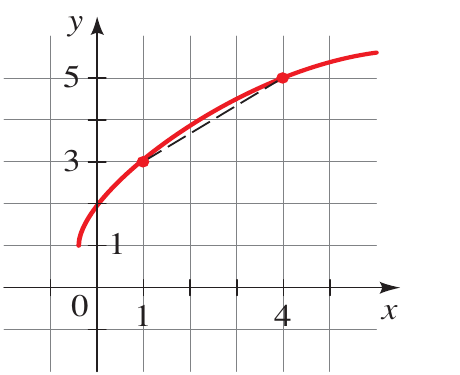
\includegraphics[width=0.42\textwidth]{fig_p04_07.png}\end{center}
\end{quote}

\begin{paso}{Paso 1 --- Leer los dos puntos marcados en la gráfica}
\textbf{Qué hago:} localizo en la gráfica las ordenadas correspondientes a $x=1$ y $x=4$ (los dos puntos rojos, extremos de la secante punteada).

\textbf{¿De dónde sale?} De las marcas del eje $x$ ($1$ y $4$) y de las rectas guía del eje $y$ ($3$ y $5$).

\textbf{¿Por qué?} La gráfica es la definición de $f$ en este ejercicio; no hay fórmula que sustituir.
\[
f(1)=3,\qquad f(4)=5.
\]
\end{paso}

\begin{paso}{Paso 2 --- Cambio neto}
\textbf{Qué hago:} resto $f(4)-f(1)$ con los valores del paso 1.

\textbf{¿Por qué?} El cambio neto de $f$ entre $x=a$ y $x=b$ se define como $f(b)-f(a)$.
\[
f(4)-f(1)=5-3=2.
\]
\end{paso}

\begin{paso}{Paso 3 --- Razón de cambio promedio}
\textbf{Qué hago:} divido el cambio neto entre el cambio en $x$, que es $4-1=3$.

\textbf{¿Por qué?} Es la pendiente de la secante punteada dibujada entre los dos puntos rojos.
\[
\frac{f(4)-f(1)}{4-1}=\frac{2}{3}.
\]
\end{paso}

\begin{resp}
\textbf{a)} Cambio neto $=2$. \qquad \textbf{b)} Razón de cambio promedio $=\dfrac{2}{3}$ (positiva, porque $f$ es creciente en $[1,4]$).
\end{resp}

% =====================================================================
\subsection*{Ejercicio 4 — Razón de cambio negativa desde la gráfica (libro 2.4 \#9, p. 188)}

\begin{quote}
\textbf{9.}
\begin{center}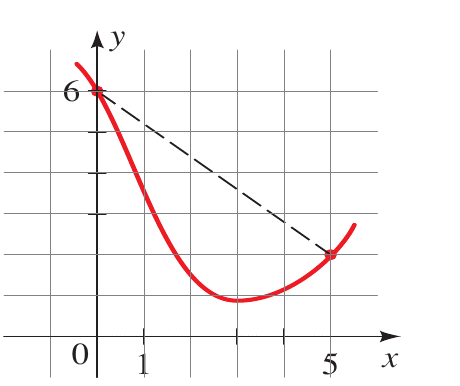
\includegraphics[width=0.42\textwidth]{fig_p04_09.png}\end{center}
\end{quote}

\begin{paso}{Paso 1 --- Leer los dos puntos marcados}
\textbf{Qué hago:} leo las ordenadas en $x=0$ y $x=5$, los extremos de la secante punteada.

\textbf{¿De dónde sale?} El punto izquierdo está sobre la marca $6$ del eje $y$; contando cuadrículas de una unidad, el punto derecho está a la altura $2$.

\textbf{¿Por qué?} La cuadrícula fija la escala: cada línea horizontal vale una unidad de $y$.
\[
f(0)=6,\qquad f(5)=2.
\]
\end{paso}

\begin{paso}{Paso 2 --- Cambio neto y razón de cambio promedio}
\textbf{Qué hago:} resto y luego divido entre $5-0=5$.

\textbf{¿Por qué?} Definición de cambio neto $f(b)-f(a)$ y de razón de cambio promedio $\dfrac{f(b)-f(a)}{b-a}$.
\[
f(5)-f(0)=2-6=-4,\qquad \frac{-4}{5-0}=-\frac{4}{5}.
\]
\end{paso}

\begin{resp}
\textbf{a)} Cambio neto $=-4$. \qquad \textbf{b)} Razón de cambio promedio $=-\dfrac{4}{5}=-0.8$; es negativa porque $f(5)<f(0)$, es decir, la función bajó en el intervalo.
\end{resp}

% =====================================================================
\subsection*{Ejercicio 5 — Razón de cambio de una función lineal (libro 2.4 \#11, p. 188)}

\begin{quote}
\textbf{11--24 $\blacksquare$ Cambio neto y razón de cambio promedio} \; Se da una función. Determine \emph{a}) el cambio neto y \emph{b}) la razón de cambio promedio entre los dos valores dados de la variable.

\textbf{11.} $f(x)=3x-2;\quad x=2,\;x=3$
\end{quote}

\begin{paso}{Paso 1 --- Evaluar en los extremos}
\textbf{Qué hago:} sustituyo $x=2$ y $x=3$ en $f(x)=3x-2$.

\textbf{¿Por qué?} La razón de cambio promedio se calcula con las imágenes, no con las entradas.
\[
f(2)=3(2)-2=4,\qquad f(3)=3(3)-2=7.
\]
\end{paso}

\begin{paso}{Paso 2 --- Cambio neto y cociente}
\textbf{Qué hago:} resto $f(3)-f(2)$ y divido entre $3-2$.

\textbf{¿Por qué?} Definición; el resultado debe coincidir con la pendiente $m=3$ por ser $f$ lineal.
\[
f(3)-f(2)=7-4=3,\qquad \frac{3}{3-2}=\frac{3}{1}=3.
\]
\end{paso}

\begin{resp}
\textbf{a)} Cambio neto $=3$. \qquad \textbf{b)} Razón de cambio promedio $=3$, igual a la pendiente de $f(x)=3x-2$.
\end{resp}

% =====================================================================
\subsection*{Ejercicio 6 — Razón de cambio de una cuadrática (libro 2.4 \#15, p. 188)}

\begin{quote}
\textbf{15.} $h(t)=2t^2-t;\quad t=3,\;t=6$
\end{quote}

\begin{paso}{Paso 1 --- Evaluar $h$ en $t=3$ y $t=6$}
\textbf{Qué hago:} sustituyo cada valor en $h(t)=2t^2-t$, respetando que el cuadrado se calcula antes de multiplicar por $2$.

\textbf{¿Por qué?} Jerarquía de operaciones: potencia, luego producto, luego resta.
\[
h(3)=2(3)^2-3=18-3=15,\qquad h(6)=2(6)^2-6=72-6=66.
\]
\end{paso}

\begin{paso}{Paso 2 --- Cambio neto y razón de cambio promedio}
\textbf{Qué hago:} resto $h(6)-h(3)$ y divido entre $6-3$.

\textbf{¿Por qué?} Definición de cambio neto y de razón de cambio promedio.
\[
h(6)-h(3)=66-15=51,\qquad \frac{51}{6-3}=\frac{51}{3}=17.
\]
\end{paso}

\begin{resp}
\textbf{a)} Cambio neto $=51$. \qquad \textbf{b)} Razón de cambio promedio $=17$.
\end{resp}

% =====================================================================
\subsection*{Ejercicio 7 — Razón de cambio de una cúbica (libro 2.4 \#17, p. 188)}

\begin{quote}
\textbf{17.} $f(x)=x^3-4x^2;\quad x=0,\;x=10$
\end{quote}

\begin{paso}{Paso 1 --- Evaluar $f$ en los extremos}
\textbf{Qué hago:} sustituyo $x=0$ y $x=10$ en $f(x)=x^3-4x^2$.

\textbf{¿Por qué?} Definición de la notación $f(x)$: se reemplaza la variable por el valor dado.
\[
f(0)=0^3-4(0)^2=0,\qquad f(10)=10^3-4(10)^2=1000-400=600.
\]
\end{paso}

\begin{paso}{Paso 2 --- Cambio neto y cociente}
\textbf{Qué hago:} resto y divido entre $10-0$.

\textbf{¿Por qué?} Definición de razón de cambio promedio.
\[
f(10)-f(0)=600-0=600,\qquad \frac{600}{10-0}=60.
\]
\end{paso}

\begin{resp}
\textbf{a)} Cambio neto $=600$. \qquad \textbf{b)} Razón de cambio promedio $=60$.
\end{resp}

% =====================================================================
\subsection*{Ejercicio 8 — Cociente de diferencias con incremento $h$ (libro 2.4 \#19, p. 188)}

\begin{quote}
\textbf{19.} $f(t)=5t^2;\quad t=3,\;t=3+h$
\end{quote}

\begin{paso}{Paso 1 --- Evaluar $f$ en $t=3$ y en $t=3+h$}
\textbf{Qué hago:} sustituyo y desarrollo $(3+h)^2$ con el cuadrado de binomio.

\textbf{¿De dónde sale?} De $f(t)=5t^2$ y de $(a+h)^2=a^2+2ah+h^2$ con $a=3$.

\textbf{¿Por qué?} Hay que dejar el numerador como polinomio para poder cancelar $h$ después.
\[
f(3)=5(3)^2=45,\qquad f(3+h)=5(3+h)^2=5(9+6h+h^2)=45+30h+5h^2.
\]
\end{paso}

\begin{paso}{Paso 2 --- Cambio neto: restar y factorizar $h$}
\textbf{Qué hago:} resto $f(3+h)-f(3)$ y saco factor común $5h$.

\textbf{¿Por qué?} El término constante $45$ se cancela, y todo lo que queda contiene el factor $h$.
\[
f(3+h)-f(3)=(45+30h+5h^2)-45=30h+5h^2=5h(6+h).
\]
\end{paso}

\begin{paso}{Paso 3 --- Dividir entre el cambio en $t$}
\textbf{Qué hago:} divido entre $(3+h)-3=h$ y cancelo el factor $h$.

\textbf{¿Por qué?} La cancelación es válida porque $h\neq 0$ (si $h=0$ los dos puntos coinciden y no hay intervalo).
\[
\frac{5h(6+h)}{h}=5(6+h)=30+5h.
\]
\end{paso}

\begin{resp}
\textbf{a)} Cambio neto $=5h(6+h)=30h+5h^2$. \qquad \textbf{b)} Razón de cambio promedio $=5(6+h)=30+5h$, con $h\neq 0$.
\end{resp}

% =====================================================================
\subsection*{Ejercicio 9 — Razón de cambio de $g(x)=1/x$ (libro 2.4 \#21, p. 188)}

\begin{quote}
\textbf{21.} $g(x)=\dfrac{1}{x};\quad x=1,\;x=a$
\end{quote}

\begin{paso}{Paso 1 --- Evaluar y restar}
\textbf{Qué hago:} calculo $g(a)-g(1)$ y junto las dos fracciones con denominador común $a$.

\textbf{¿De dónde sale?} De $g(x)=1/x$: $g(1)=1/1=1$ y $g(a)=1/a$.

\textbf{¿Por qué?} Sumar/restar fracciones exige denominador común antes de simplificar.
\[
g(a)-g(1)=\frac{1}{a}-1=\frac{1-a}{a}.
\]
\end{paso}

\begin{paso}{Paso 2 --- Dividir entre $a-1$ y cancelar}
\textbf{Qué hago:} divido entre el cambio en $x$, que es $a-1$, y uso $1-a=-(a-1)$ para cancelar.

\textbf{¿Por qué?} La cancelación de $a-1$ vale porque $a\neq 1$; si $a=1$ los dos puntos coinciden.
\[
\frac{\dfrac{1-a}{a}}{a-1}=\frac{1-a}{a(a-1)}=\frac{-(a-1)}{a(a-1)}=-\frac{1}{a}.
\]
\end{paso}

\begin{resp}
\textbf{a)} Cambio neto $=\dfrac{1-a}{a}$. \qquad \textbf{b)} Razón de cambio promedio $=-\dfrac{1}{a}$, válida para $a\neq 0$ y $a\neq 1$.
\end{resp}

% =====================================================================
\subsection*{Ejercicio 10 — Cociente de diferencias de $f(t)=2/t$ (libro 2.4 \#23, p. 188)}

\begin{quote}
\textbf{23.} $f(t)=\dfrac{2}{t};\quad t=a,\;t=a+h$
\end{quote}

\begin{paso}{Paso 1 --- Restar las dos fracciones}
\textbf{Qué hago:} calculo $f(a+h)-f(a)$ con denominador común $a(a+h)$.

\textbf{¿De dónde sale?} De $f(t)=2/t$: $f(a)=\dfrac{2}{a}$ y $f(a+h)=\dfrac{2}{a+h}$.

\textbf{¿Por qué?} Es el único modo de simplificar la resta hasta ver el factor $h$.
\[
\frac{2}{a+h}-\frac{2}{a}=\frac{2a-2(a+h)}{a(a+h)}=\frac{2a-2a-2h}{a(a+h)}=\frac{-2h}{a(a+h)}.
\]
\end{paso}

\begin{paso}{Paso 2 --- Dividir entre $h$}
\textbf{Qué hago:} divido el cambio neto entre $(a+h)-a=h$ y cancelo $h$.

\textbf{¿Por qué?} Cancelar $h$ es lícito porque $h\neq 0$; el resultado ya no tiene $h$ en el numerador.
\[
\frac{1}{h}\cdot\frac{-2h}{a(a+h)}=\frac{-2}{a(a+h)}.
\]
\end{paso}

\begin{resp}
\textbf{a)} Cambio neto $=\dfrac{-2h}{a(a+h)}$. \qquad \textbf{b)} Razón de cambio promedio $=-\dfrac{2}{a(a+h)}$, con $a\neq 0$, $a+h\neq 0$ y $h\neq 0$.
\end{resp}

% =====================================================================
\subsection*{Ejercicio 11 — Razón de cambio constante de una lineal (libro 2.4 \#25, p. 188)}

\begin{quote}
\textbf{25--26 $\blacksquare$ Razón de cambio promedio de una función lineal} \; Se da una función lineal. \emph{a}) Determine la razón de cambio promedio de la función entre $x=a$ y $x=a+h$. \emph{b}) Demuestre que la razón de cambio promedio es igual que la pendiente de la recta.

\textbf{25.} $f(x)=\tfrac{1}{2}x+3$
\end{quote}

\begin{paso}{Paso 1 --- Evaluar en $x=a$ y $x=a+h$}
\textbf{Qué hago:} sustituyo ambos valores en $f(x)=\tfrac12 x+3$ y distribuyo $\tfrac12$.

\textbf{¿Por qué?} Propiedad distributiva: $\tfrac12(a+h)=\tfrac12 a+\tfrac12 h$.
\[
f(a)=\tfrac12 a+3,\qquad f(a+h)=\tfrac12(a+h)+3=\tfrac12 a+\tfrac12 h+3.
\]
\end{paso}

\begin{paso}{Paso 2 --- Cociente de diferencias}
\textbf{Qué hago:} resto y divido entre $(a+h)-a=h$; los términos $\tfrac12 a$ y $3$ se cancelan.

\textbf{¿Por qué?} Definición de razón de cambio promedio; se cancela $h$ porque $h\neq 0$.
\[
\frac{\left(\tfrac12 a+\tfrac12 h+3\right)-\left(\tfrac12 a+3\right)}{h}=\frac{\tfrac12 h}{h}=\frac{1}{2}.
\]
\end{paso}

\begin{paso}{Paso 3 --- Inciso b): comparar con la pendiente}
\textbf{Qué hago:} identifico la pendiente de $f(x)=\tfrac12 x+3$ leyendo el coeficiente de $x$.

\textbf{¿Por qué?} En la forma pendiente-intersección $f(x)=mx+b$, la pendiente es $m$; aquí $m=\tfrac12$, que es exactamente el valor del paso 2.
\end{paso}

\begin{resp}
\textbf{a)} La razón de cambio promedio entre $x=a$ y $x=a+h$ es $\tfrac12$, sin depender de $a$ ni de $h$.\\
\textbf{b)} Coincide con la pendiente $m=\tfrac12$ de la recta $y=\tfrac12 x+3$: una función lineal tiene razón de cambio constante.
\end{resp}

% =====================================================================
\subsection*{Ejercicio 12 — Comparación de razones de cambio en gráficas (libro 2.4 \#28, p. 188)}

\begin{quote}
\textbf{28. Razón de cambio promedio} \; A continuación se muestran las gráficas de las funciones $f$, $g$ y $h$. ¿Qué puede decir acerca de la razón de cambio promedio de cada función en los intervalos sucesivos $[0,1]$, $[1,2]$, $[2,3]$, \ldots?

\begin{center}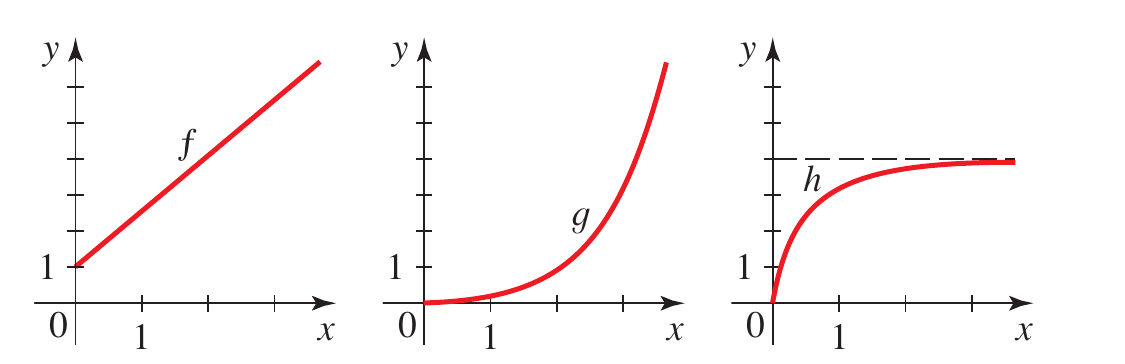
\includegraphics[width=0.92\textwidth]{fig_p04_28.png}\end{center}
\end{quote}

\begin{paso}{Paso 1 --- Traducir la pregunta a pendientes de secantes}
\textbf{Qué hago:} en cada intervalo de longitud $1$ la razón de cambio promedio es $\dfrac{F(n+1)-F(n)}{1}=F(n+1)-F(n)$, o sea la pendiente de la secante entre dos marcas consecutivas.

\textbf{¿Por qué?} Como $b-a=1$, la razón de cambio promedio se reduce al cambio neto en ese intervalo.
\end{paso}

\begin{paso}{Paso 2 --- Gráfica de $f$: recta}
\textbf{Qué hago:} observo que la gráfica de $f$ es una recta, así que todas las secantes tienen la misma pendiente.

\textbf{¿Por qué?} Una función lineal tiene razón de cambio constante (resultado del ejemplo 4 de la sección).
\end{paso}

\begin{paso}{Paso 3 --- Gráfica de $g$: crece cada vez más rápido}
\textbf{Qué hago:} comparo los saltos verticales de $g$ en $[0,1]$, $[1,2]$, $[2,3]$: cada uno es mayor que el anterior.

\textbf{¿Por qué?} La curva se empina hacia la derecha, luego las secantes sucesivas tienen pendiente cada vez mayor: las razones de cambio promedio son positivas y crecientes.
\end{paso}

\begin{paso}{Paso 4 --- Gráfica de $h$: crece cada vez más lento}
\textbf{Qué hago:} comparo los saltos verticales de $h$: cada uno es menor que el anterior y se aproximan a $0$.

\textbf{¿Por qué?} La curva se aplana hacia la asíntota horizontal punteada, luego las secantes son positivas pero de pendiente cada vez menor.
\end{paso}

\begin{resp}
En los intervalos sucesivos $[0,1]$, $[1,2]$, $[2,3]$, \ldots:
\begin{itemize}[leftmargin=*]
  \item $f$: razón de cambio promedio \textbf{constante} (positiva), porque su gráfica es una recta.
  \item $g$: razones positivas y \textbf{crecientes}, porque la curva se empina.
  \item $h$: razones positivas y \textbf{decrecientes}, tendiendo a $0$, porque la curva se aplana hacia su asíntota horizontal.
\end{itemize}
\end{resp}

% =====================================================================
\subsection*{Ejercicio 13 — Cambio de niveles de agua (libro 2.4 \#29, p. 188)}

\begin{quote}
\textbf{29. Cambio de niveles de agua} \; La gráfica muestra la profundidad del agua $W$ en un depósito en un periodo de un año como función del número de días $x$ desde el principio del año. ¿Cuál fue la razón de cambio promedio de $W$ entre $x=100$ y $x=200$?

\begin{center}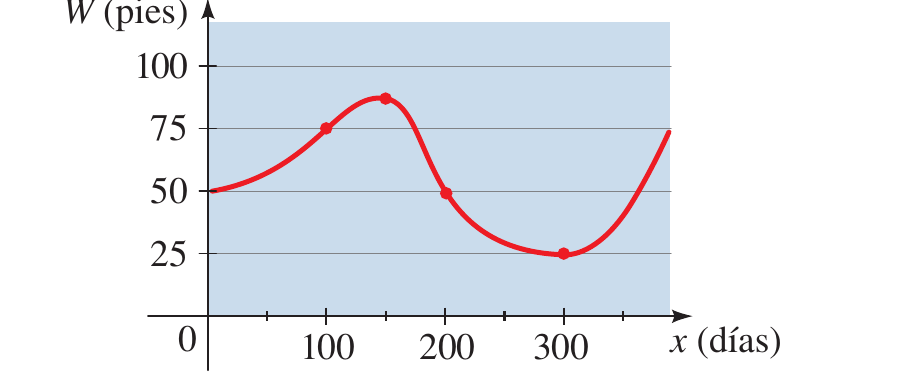
\includegraphics[width=0.6\textwidth]{fig_p04_29.png}\end{center}
\end{quote}

\begin{paso}{Paso 1 --- Leer $W(100)$ y $W(200)$ en la gráfica}
\textbf{Qué hago:} localizo en la curva los puntos marcados sobre $x=100$ y $x=200$ y leo su altura en el eje $W$.

\textbf{¿De dónde sale?} De las líneas horizontales de referencia del eje $W$, rotuladas $25$, $50$, $75$, $100$.

\textbf{¿Por qué?} La gráfica define la función; no hay fórmula para $W$.
\[
W(100)=75\ \text{pies},\qquad W(200)=50\ \text{pies}.
\]
\end{paso}

\begin{paso}{Paso 2 --- Aplicar la fórmula con unidades}
\textbf{Qué hago:} divido el cambio neto entre el tiempo transcurrido $200-100=100$ días.

\textbf{¿Por qué?} Definición de razón de cambio promedio; las unidades son pies por día.
\[
\frac{W(200)-W(100)}{200-100}=\frac{50-75}{100}=\frac{-25}{100}=-0.25.
\]
\end{paso}

\begin{resp}
La razón de cambio promedio fue $-0.25$ pies por día (el nivel bajó, en promedio, un cuarto de pie diario entre el día 100 y el día 200).
\end{resp}

% =====================================================================
\subsection*{Ejercicio 14 — Crecimiento y decrecimiento de la población (libro 2.4 \#31, p. 189)}

\begin{quote}
\textbf{31. Crecimiento y decrecimiento de la población} \; La tabla da la población en una pequeña comunidad costera para el periodo 1997-2006. Las cifras que se muestran son para el 1 de enero de cada año.

\emph{a}) ¿Cuál fue la razón de cambio promedio de la población entre 1998 y 2001?

\emph{b}) ¿Cuál fue la razón de cambio promedio de la población entre 2002 y 2004?

\emph{c}) ¿Para qué periodo fue creciente la población?

\emph{d}) ¿Para qué periodo fue decreciente la población?

\begin{center}
\begin{tabular}{|c|c|}
\hline
\textbf{Año} & \textbf{Población}\\
\hline
1997 & 624\\
1998 & 856\\
1999 & 1\,336\\
2000 & 1\,578\\
2001 & 1\,591\\
2002 & 1\,483\\
2003 & 994\\
2004 & 826\\
2005 & 801\\
2006 & 745\\
\hline
\end{tabular}
\end{center}
\end{quote}

\begin{paso}{Paso 1 --- Inciso a): tomar los datos de 1998 y 2001}
\textbf{Qué hago:} leo $P(1998)=856$ y $P(2001)=1\,591$ en la tabla y aplico la fórmula con $b-a=2001-1998=3$ años.

\textbf{¿Por qué?} Definición de razón de cambio promedio: cambio neto de población entre años transcurridos.
\[
\frac{P(2001)-P(1998)}{2001-1998}=\frac{1591-856}{3}=\frac{735}{3}=245.
\]
\end{paso}

\begin{paso}{Paso 2 --- Inciso b): datos de 2002 y 2004}
\textbf{Qué hago:} leo $P(2002)=1\,483$ y $P(2004)=826$ y divido entre $2004-2002=2$ años.

\textbf{¿Por qué?} Misma definición; el signo negativo indicará que la población disminuyó.
\[
\frac{P(2004)-P(2002)}{2004-2002}=\frac{826-1483}{2}=\frac{-657}{2}=-328.5.
\]
\end{paso}

\begin{paso}{Paso 3 --- Incisos c) y d): comparar valores consecutivos}
\textbf{Qué hago:} recorro la columna de población y veo dónde los valores suben y dónde bajan.

\textbf{¿Por qué?} Una función es creciente donde cada valor supera al anterior y decreciente donde cada valor es menor que el anterior.
\[
624<856<1336<1578<1591>1483>994>826>801>745.
\]
\end{paso}

\begin{resp}
\textbf{a)} $245$ personas por año. \qquad \textbf{b)} $-328.5$ personas por año (la población disminuyó).\\
\textbf{c)} Creciente de 1997 a 2001. \qquad \textbf{d)} Decreciente de 2001 a 2006.
\end{resp}

% =====================================================================
\subsection*{Ejercicio 15 — Ventas de reproductores de DVD (libro 2.4 \#33, p. 189)}

\begin{quote}
\textbf{33. Ventas de reproductores de DVD} \; La tabla siguiente muestra el número de reproductores de DVD vendidos en una pequeña tienda de aparatos electrónicos en los años 2003-2013.

\emph{a}) ¿Cuál fue la razón de cambio promedio de ventas entre 2003 y 2013?

\emph{b}) ¿Cuál fue la razón de cambio promedio de ventas entre 2003 y 2004?

\emph{c}) ¿Cuál fue la razón de cambio promedio de ventas entre 2004 y 2005?

\emph{d}) ¿Entre cuáles dos años sucesivos las ventas de reproductores de DVD \emph{aumentaron} más rápidamente? ¿Entre cuáles \emph{disminuyeron} más rápidamente?

\begin{center}
\begin{tabular}{|c|c|}
\hline
\textbf{Año} & \textbf{Reproductores de DVD vendidos}\\
\hline
2003 & 495\\
2004 & 513\\
2005 & 410\\
2006 & 402\\
2007 & 520\\
2008 & 580\\
2009 & 631\\
2010 & 719\\
2011 & 624\\
2012 & 582\\
2013 & 635\\
\hline
\end{tabular}
\end{center}
\end{quote}

\begin{paso}{Paso 1 --- Inciso a): intervalo 2003--2013}
\textbf{Qué hago:} tomo $V(2003)=495$ y $V(2013)=635$ y divido entre $2013-2003=10$ años.

\textbf{¿Por qué?} Definición de razón de cambio promedio; las unidades son reproductores por año.
\[
\frac{635-495}{10}=\frac{140}{10}=14.
\]
\end{paso}

\begin{paso}{Paso 2 --- Incisos b) y c): intervalos de un año}
\textbf{Qué hago:} aplico la fórmula con $b-a=1$, de modo que la razón coincide con el cambio neto.

\textbf{¿Por qué?} Al dividir entre $1$ el cociente no altera el numerador.
\[
\frac{513-495}{2004-2003}=\frac{18}{1}=18,\qquad
\frac{410-513}{2005-2004}=\frac{-103}{1}=-103.
\]
\end{paso}

\begin{paso}{Paso 3 --- Inciso d): comparar los cambios año a año}
\textbf{Qué hago:} calculo todas las diferencias entre años consecutivos y busco la mayor y la menor.

\textbf{¿Por qué?} Todos los intervalos miden $1$ año, así que comparar razones equivale a comparar cambios netos.
\[
\begin{array}{ll}
+18\;(03\text{--}04), & -103\;(04\text{--}05),\; -8\;(05\text{--}06),\; +118\;(06\text{--}07),\; +60\;(07\text{--}08),\\
+51\;(08\text{--}09), & +88\;(09\text{--}10),\; -95\;(10\text{--}11),\; -42\;(11\text{--}12),\; +53\;(12\text{--}13).
\end{array}
\]
\end{paso}

\begin{resp}
\textbf{a)} $14$ reproductores por año. \quad \textbf{b)} $18$ por año. \quad \textbf{c)} $-103$ por año.\\
\textbf{d)} Aumentaron más rápidamente entre \textbf{2006 y 2007} ($+118$); disminuyeron más rápidamente entre \textbf{2004 y 2005} ($-103$).
\end{resp}

\end{document}
